INTRODUCTION

\chapter{General Overview}

Since the beginning of time life has made its way through multiple adverse conditions. Organisms have evolved from single cells interacting directly with their environment, to specialised multicellular entities that respond specifically to different stimuli. Even though cells can specialise their functions by differentiating into diverse cell-types, by aggregating into tissues, generating organs and/or forming a variety of organisms, they all respond to the same paradigm. DNA is used to save and protect the hereditary information, which is later transcribed into functional orders in the form of RNA, being most of the time translated into protein products that execute those final orders.

This process was broadly studied in the twentieth century in order to explain how life works. DNA was discovered to be the main source of information, in a double helix format, carrying and saving all necessary instructions to secure life over generations \citep{watson1953molecular}. It was discovered a few years later that the incorporation of the deoxyribonucleotides, from the triphosphates of deoxyadenosine, deoxyguanosine, deoxycytidine and thymidine, into the deoxyribonucleic acid was catalysed by an enzyme, the DNA polymerase, which was purified at that time directly from \textit{Escherichia coli} cell-free extracts \citep{lehman1958enzymatic}. 

Proteins were further investigated as the final output of DNA's translation of information, backed by the discovery of the green fluorescent protein (GFP), purified for the first time from the \textit{Aequorea victoria} jellyfish \citep{shimomura1962extraction}, which allowed tracking and detection of fusion proteins in real-time. Shimomura's achievement was inspired by the work carried out by \citet{dubois1885fonction} where crude extracts from an Elaterid, \textit{Pyrophorus}, and a Clam, \textit{Pholas}, made possible the generation of luminescence in solutions containing dissolved oxygen, now known as the luciferin-luciferase reaction and one of the first instances where enzymatic functionality was proved in vitro. 

Even though the first enzyme was discovered by \citet{payen1833memoir}, at that time they were known as "ferments" and mentioned by Louis Pasteur as "responsible for fermentation but strongly dependent on living organisms, as without  live  yeast,  no  fermentation  can exist". This assumption was based on his unsuccessful attempt to isolate the mentioned active principle from living yeasts \citep{manchester1995louis}. It was not until 40 years later that the term enzyme was used \citep{kuhne1877behavior} and made popular by \citet{buchner1897alkoholische} who found that sugar was fermented by yeast extracts even when there was no living yeast cells in the mixture (Figure \ref{fig.intro1}), thus achieving the first cell-free fermentation, to which he added later works with coagulases, catalases, lactases and toluene degrading extracts \citep{buchner1907cell}. 

\begin{figure}[htb]
  \centering
  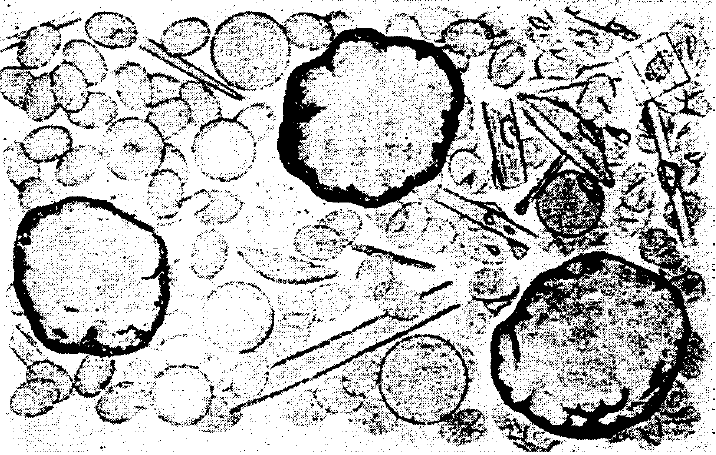
\includegraphics[width=0.7\textwidth]{introduction/chapter/figs/cells_extract.png}
  \caption{Diagrammatic representation of the crushing process: yeast ground with quartz sand and diatomite until the cells burst, the contents thereof emerging in the form of mucous lumps from the cell membrane. Illustration reproduced from \citet{buchner1907cell}}
  \label{fig.intro1}
\end{figure}


Endonucleases were another type of enzyme that revolutionised molecular biology. Endonucleases were discovered in the early 1960s \citep{arber1962host} by using one-step lysates from a $\lambda$ and/or P1 phage infected non-lysogenic \textit{Escherichia coli} K12 bacteria. Recognised as the "molecular scissors" protecting bacteria from bacteriophages, these restriction enzymes working in conjunction with methylases were capable of protecting the DNA of bacteria. Since the isolation of the first endonuclease from dialysed lysates of \textit{Escherichia coli} K, these started to be called restriction enzymes for their ability to "restrict" entrance of foreign genetic material, cutting it in as little as 10 to 30 seconds \citep{meselson1968dna}. Their specificity was later confirmed by \citet{kelly1970restriction} who described the 6 bp specific cleavage site of an endonuclease isolated from \textit{Haemophilus influenzae Rd} (Figure \ref{fig.intro2}). Enzyme later named as HindII by using the genus and species name of the host organism in a three-letter code, followed by the strain or type identification \citep{smith1973suggested}. The understanding of how restriction enzymes cut DNA, and how host DNA tries to protect itself became the basis of modern genetic engineering. 

\begin{figure}[!ht]
  \centering
  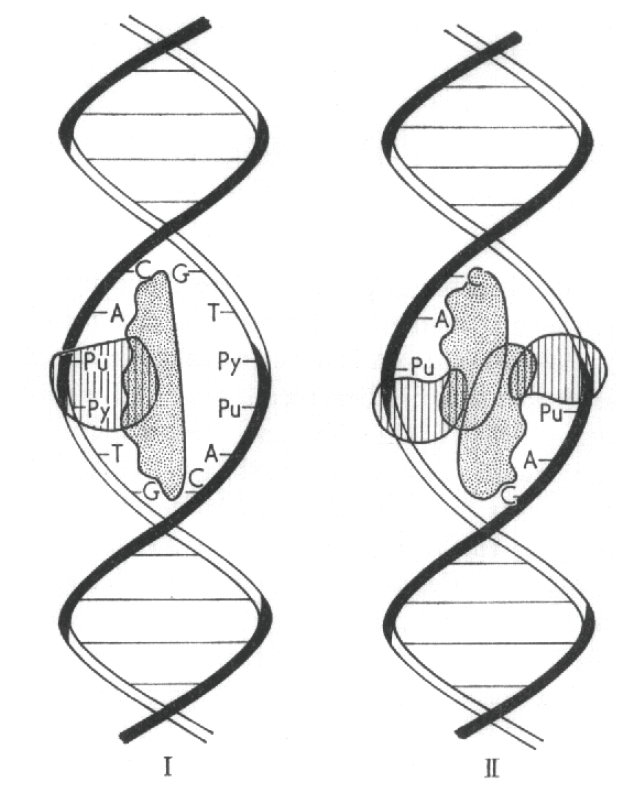
\includegraphics[width=0.7\textwidth]{introduction/chapter/figs/dnase.png}
  \caption{Recognition of a symmetrical nucleotide sequence by endonuclease R. Two possible models. Model I. A single enzyme molecule specifically binds to the base sequence GpTpPypPupApC.The active site of the enzyme (shaded area) catalyzes 5’-phosphoryl, 3’-hydroxyl cleavage of the phosphodiester bond between Py and Pu. The enzyme then detaches and attacks the other strand which (because of symmetry) contains the same base sequence. An even duplex break results. (Note: since endonuclease R is inactive on single-stranded DNA, it is necessary to assume in this model that the enzyme in some way “senses” the bihelical configuration of the substrate). 
  Model II. The enzyme is composed of two identical subunits (related by a g-fold rotational axis of symmetry) which bind to the sequence pPupApC on opposite strands of the DNA duplex. Each subunit is actually a dimer constructed from a “recognition” subunit (stippled) and a "nuclease" subunit (shaded). The recognition subunits bind to A and C, while the nuclease subunits bind to Pu. Hydrolysis of the phosphodiester bonds between Py and Pu by the nuclease subunits results in a duplex break. Illustration reproduced from \citet{kelly1970restriction}}
  \label{fig.intro2}
\end{figure}

Recombinant DNA molecules were created for the first time by the fusion of genetic material from more than one species \citep{jackson1972biochemical}. Here the DNA from two viruses, SV40 and $\lambda$, and the galactose operon of \textit{E. coli}  was cut creating “sticky ends” and the ends annealed and sealed with the addition of DNA polymerase and DNA ligase, forming one covalently closed-circular DNA molecule (Figure \ref{fig.intro3}). This was further confirmed by observing via gel electrophoresis, and comparing with previous SV40 viral genome observations performed by \citet{danna1971specific}, who created this now well-known visualization technique (Figure \ref{fig.intro4}), and gave a vital foundation for the later generation of genomic mapping.

\begin{figure}[!ht]
  \centering
  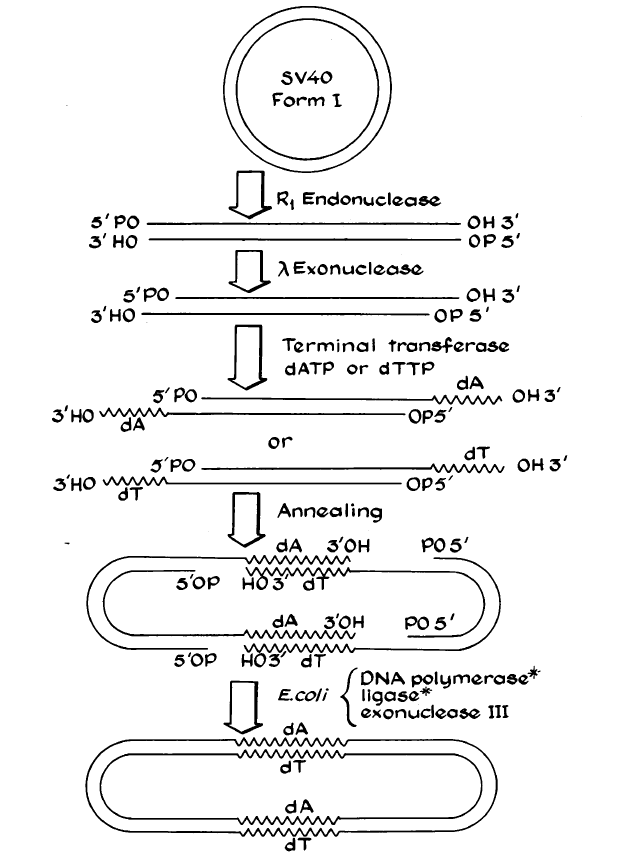
\includegraphics[width=0.7\textwidth]{introduction/chapter/figs/recombinant.png}
  \caption{General protocol for producing covalently closed
SV40 dimer circles from SV40(I) DNA. *The four deoxynucleoside triphosphates and NAD are also present for the DNA polymerase and ligase reactions, respectively. Illustration reproduced from \citet{jackson1972biochemical}}
  \label{fig.intro3}
\end{figure}

The introduction of recombinant DNA into living organisms was achieved by \citet{cohen1973construction}, proving that DNA can not only replicate naturally, despite being artificially introduced into another organism, but also can ligate in vivo. Since this work also proved that reassociated molecules carrying antibiotic resistance genes are capable of replication, can circularize and can be recovered as functional plasmids by appropriate selection, it establishes the principles of recombinant DNA technology and opens a new era of scientific discovery. 

A novel method for determining nucleotide sequences in DNA was described by \citet{sanger1977dna} making use of the 2',3'-dideoxy and arabinonucleoside analogues of the normal deoxynucleoside triphosphates, which act as specific chain-terminating inhibitors of DNA polymerase. Allowing to determine the sequence from 15 to around 200 nucleotides from the priming site with reasonable accuracy using a single primer \ref{fig.intro6}.

\begin{figure}[!ht]
  \centering
  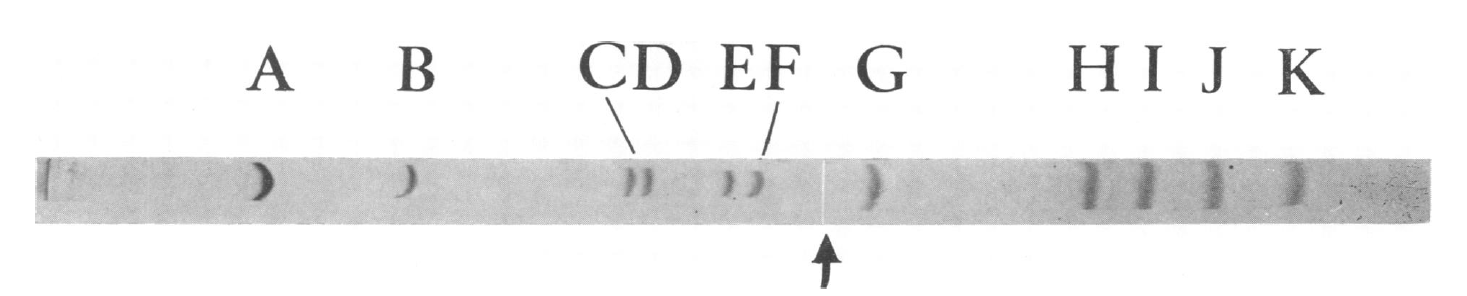
\includegraphics[width=0.7\textwidth]{introduction/chapter/figs/electrophoresis.png}
  \caption{Radioautographic analysis of SV40 DNA digested with \textit{H. influenzae} restriction endonuclease. 1 $\mu$g of SV40 [$^{14}$C]-DNA I (3 X 10$^4$ cpm/$\mu$g) was digested (see Fig. 2) for 6 hr in a volume of 55 $\mu$l; 0.0015 unit of enzyme was added at 0 time and at 1, 2, 3, 4, and 5 hr. 20 $\mu$l of sample was electrophoresed for 12.3 hr and the radioautogram was prepared as described in Methods \citep{danna1971specific}. The origin is at the left. The arrow below the radioautogram indicates a transverse cut made in the gel prior to slicing. Illustration reproduced from \citet{danna1971specific}}
  \label{fig.intro4}
\end{figure}

 As seen, molecular biology and genetic engineering have its genesis in a test tube looking for the origins of life in a liquid format; and cell extracts are present since their inception, hence, also in Synthetic Biology. The first \textit{in vitro} translation via the usage of cell-extracts \citep{miller1970visualization} demonstrated that RNA and protein synthesis can occur almost simultaneously in the cell, process that can be completely replicated in a test tube \ref{fig.intro7}. Thus, the usage of cell-free technology is not a new approach, and neither is Synthetic Biology. For instance, one of the first mentions of Synthetic Biology as a term can be traced back to \citet{leduc1912biologie}, who sought to synthesise life "by directing the physical forces which are its cause" and strongly stated that "It is in the physico-chemistry of liquids that an explanation of the phenomena of life is to be sought". 
The interconnection between liquids and life was a current of thought shared also by \citet{haldane1926mathematical} who proposed that the primordial sea served as a vast chemical laboratory powered by solar energy. Furthermore, \citet{oparin1924proiskhozhedenie} mentions that the first living beings found organic compounds, abiogenically formed, even highlighting that on the one hand, the synthesis of proteins requires the presence of nucleic acids while, on the other, the synthesis of nucleic acids requires the presence of proteins (enzymes).  By mixing inorganic constituents, nucleic acids and proteins, many authors looked for the ultramicroscopic particle endowed with catalytic and self-replicating properties of which the influences were able to permeate the entire cell, named at that time as genes \citep{muller1922variation}. Mixing of genes and other biomolecules would allow the synthesis of macronutrients, such as lactose achieved by Rohman (1919) by using extracts from mammary gland \citep{wasteneys1930enzymatic}. 



\begin{figure}[!ht]
  \centering
  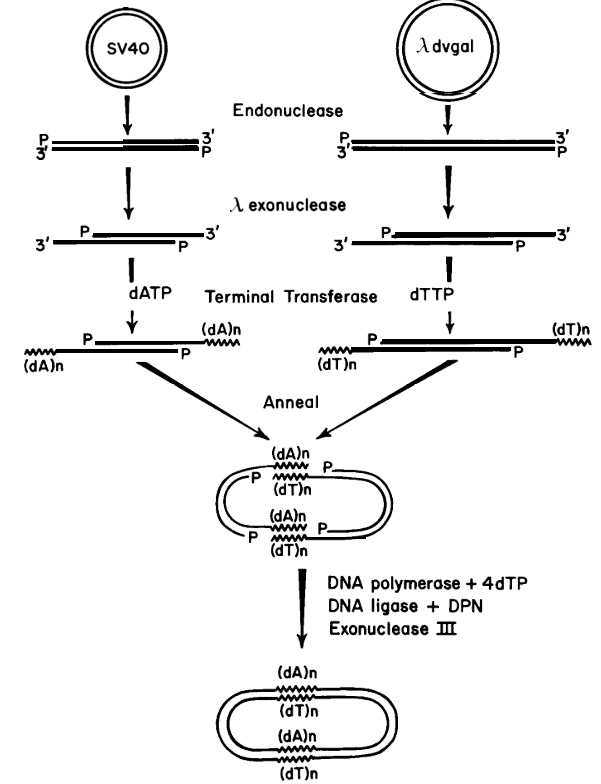
\includegraphics[width=0.7\textwidth]{introduction/chapter/figs/cohen.png}
  \caption{The construction of SV40-$\lambda\delta$ gal recombinant DNA. Illustration reproduced from \citet{berg1981dissections}}
  \label{fig.intro5}
\end{figure}

Looking for genes and the origin of life is that Teleonomy born reinstating the apparent purposefulness of structures and functions in living organisms, usually triggered by natural processes like natural selection. In 1961, after the “Cold Spring Harbor symposia on quantitative biology” \citet{monod1961general} tried to reconsider the problem of cellular regulation, summarising the discussions held and concluding that certain systems which appeared entirely different from one another are in fact submitted to similar, if not identical, controls that are in turn organised into different but also specific circuits. Basing themselves into Henri-Michaelis kinetics and Haldane equations they reintroduce mass action as one of the controlling factors in any enzyme-catalysed reaction, explaining that enzyme activity molecularly depends on their environment for their activation and inhibition (explaining competitiveness, allosteric reactions and feedbacks), molecular conversion (from zymogens to active enzymes and/or change in specificity), synthesis (associated to controlled compartments), stabilisation (connected to a wide variety of "circuits", endowed with any desired degree of stability), the gene expression that controls it (mentioning regulators, operators, operons, activators and transcriptional units) and the possible existence of an intermediate step between DNA and ribosomes, named messenger RNA, which existence was later confirmed by \citet{hurwitz1963role}. 


\begin{figure}[!ht]
  \centering
  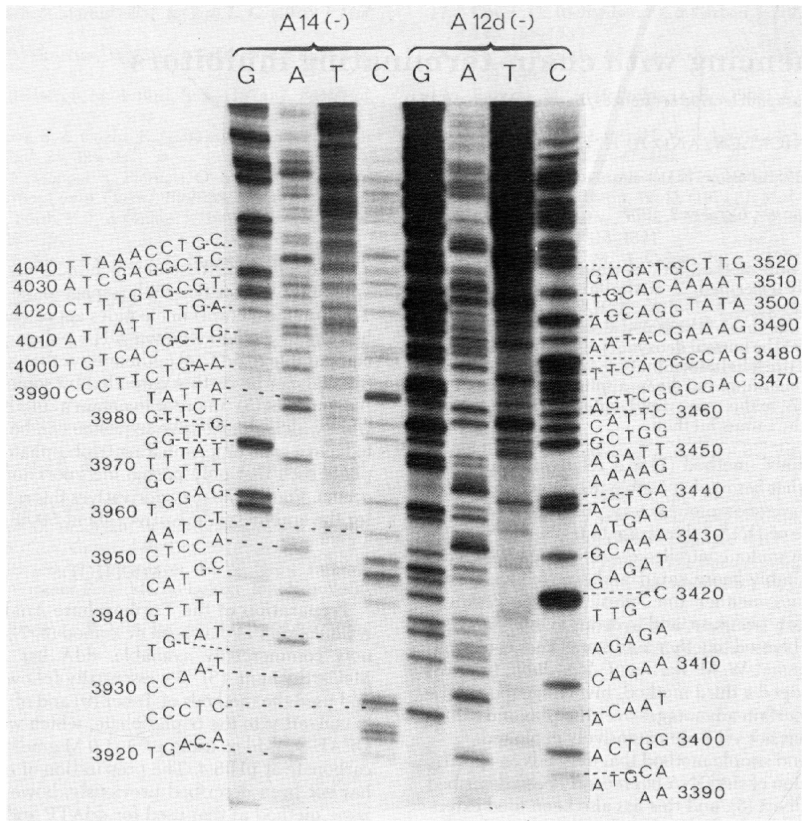
\includegraphics[width=0.7\textwidth]{introduction/chapter/figs/sanger.png}
  \caption{Autoradiograph of the acrylamide gel from the sequence determination using restriction fragments A12d and A14 as primers on the complementary strand of $\phi$X174 DNA. The inhibitor used were (left to right). The inhibitors used were (left to right) ddGTP, ddATP, ddTTP and araCTP. Electrophoresis was on a 12\% acrylamide gel at 40 mA for 14 hr. The top 10 cm of the gel is not shown. The DNA sequence is written from left to right and upwards beside the corresponding bands on the radioautograph. Illustration reproduced from \citet{sanger1977dna}}
  \label{fig.intro6}
\end{figure}

The rise of the “omics” era together with the perfectioning and widespread of complete-genome sequencing techniques led to what is currently known as Synthetic Biology \citep{cameron2014brief}, where the genetic knowledge is applied to create novel architectures going even further than what can be found in living organisms. On the start of the 21st century two synthetic genetic circuits were published, a toggle switch requiring external but transient induction instead of a sustained over time as occurs in living systems \citep{gardner2000construction} and a repressilator that uses decontextualised but naturally occurring genetic components to generate oscillatory transcriptional networks \citep{elowitz2000synthetic}.

Natural systems can be explained by studying simple synthetic circuits. For example, expression at single cell-level shows that noise plays an important role in bacteria during gene expression \citep{elowitz2002stochastic}; RNA circuits with engineered riboregulators showed the possibility to block recognition of the RBS using a \textit{cis}-repressed mRNA (crRNA) and further activation via a trans-activating RNA (taRNA) that hybridises with the crRNA, showing post-transcriptional control in both in vitro and in vivo \citep{isaacs2004engineered}; cell–cell communication and intracellular signal processing has also been explained  using synthetic multicellular consortia capable of pattern formation \citep{basu2005synthetic}; Novel discoveries in transcriptional regulation using genetic circuits allowed the generation of unnatural genetic networks \citep{alon2007network}.

Since site-specific recombination leaves short sequences in the final construct (recombination site), new cloning techniques were developed to have more accurate and efficient ways of genetic circuit generation.  Golden gate allows to create up to 256 different 4 nt overhangs using an alternative subcloning strategy that uses Type IIs restriction enzymes \citep{engler2008one}, which can cleave DNA outside of their recognition site and leave DNA overhangs consisting of any sequence allowing to clone with unique insert precision. Another assembly method that revolutionized the industry was Gibson assembly. By using a 5’ exonuclease, a DNA polymerase, and a DNA ligase this technic allows the assembly of synthetic and natural genes, genetic pathways and even entire genomes in an isothermal single reaction method \citep{gibson2009enzymatic}. 

With the advances in cloning strategies, synthetic circuits started becoming more advanced and complex. RNA devices able to execute higher-order cellular information processing operations from standard components were engineered as devices functioning as logic gates (AND, NOR, NAND, or OR gates) and signal filters, even exhibiting cooperativity \citep{win2008higher}. Multicellular biocomputing was achieved by using genetically encoded NOR gates via the generation of quorum sensing molecules by simple genetic circuits distributed in multiple cells, generating complex computation, such as XOR and EQUALS functions) in multicellular consortia \citep{tamsir2011robust}. 

Via the construction of single input–single output RNA devices, consisting of a sensor component, made of an RNA aptamer, an actuator component, made of a hammerhead ribozyme, and a transmitter component, made of a sequence that couples the sensor and actuator components, simple RNA devices that function as single-input Buffer and Inverter gates that convert a molecular input to increased and decreased gene expression output were created \citep{win2008higher}. More advances in RNA usage for genetical engineering was achieved by \cite{jinek2012programmable} revolutionising the industry. Here the system providing adaptive immunity against viruses and plasmids on bacteria and archaea was used to create a dual-RNA-guided DNA endonuclease. Clustered regularly interspaced short palindromic repeats (CRISPR) associated with the Cas endonuclease allows to cleave sequence-sepecific DNA generating an RNA programmable genome editing technic. 

\citet{paige2011rna} designed synthetic fluorescent RNA aptamers that mimic fluorescent proteins without the need for translation. The secondary structure of these aptamers presents a loop in which a fluorophore is trapped, conferring the same intramolecular immobilization that confers fluorescence in fluorescent proteins \citep{paige2011rna, strack2013superfolding}. The usage of RNA instead of proteins as output signal enhances the efficiency and response of synthetic circuits which added to recent advances in RNA technology broadens the possibility of their usage.

The expanded knowledge beyond the cell functionality created a path for the creation of Cell-free Synthetic Biology \citep{hodgman2012cell}. Cell-free expression systems are a powerful tool based in the early studies about expression originated in the 1960s-1970s with the added knowledge from current research. Cell-free systems are a powerful tool in applications where cell-based expression is too variable, slow, difficult to store or prohibitive due to legislation on the release of genetically modified organisms. 

\begin{figure}[!ht]
  \centering
  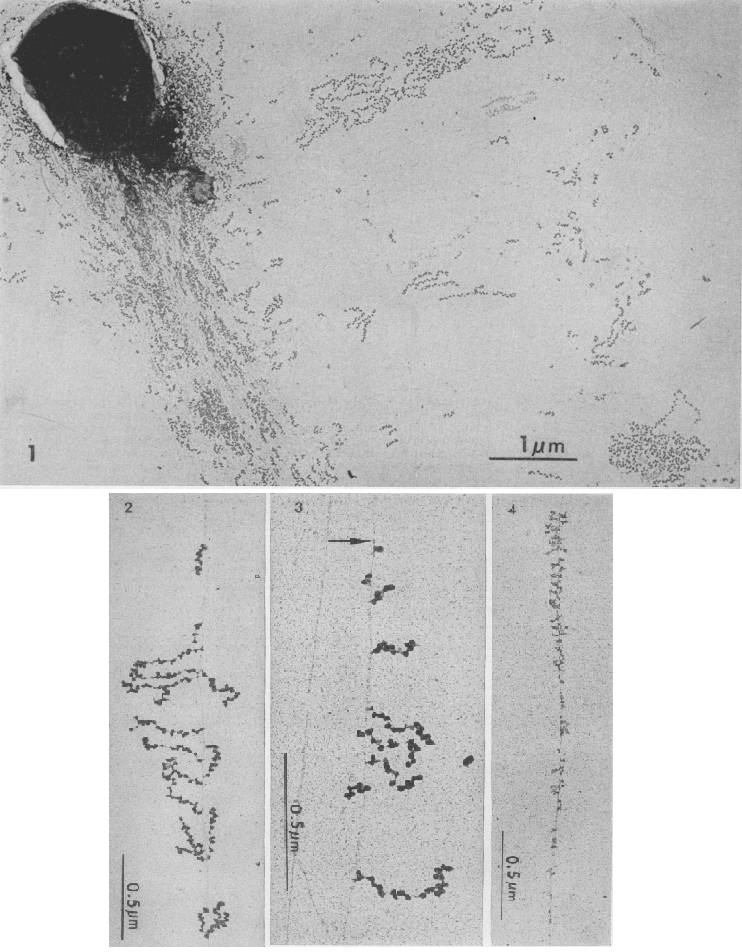
\includegraphics[width=0.7\textwidth]{introduction/chapter/figs/miller.png}
  \caption{Electron micrograph showing a portion of the extruded contents of an osmotically ruptured \textit{E. coli} cell. Fragile cells (2) were burst by rapid dilution (1:50) into distilled water adjusted to pH 9. The burst cells were immediately centrifuged (3200 rev/min at 19.3 cm radius for 3 to 5 minutes) through a O.1 M sucrose plus 10 percent formalin (pH 8.5) cushion onto carbon coated grids. The grids were rinsed in 0.4 percent Kodak Photo-flo, dried, and stained for 1 minute each in 1 percent phosphotungstic acid and 1 percent uranyl acetate, with both stains dissolved in 70 percent ethanol. The grids were then rinsed briefly in 95 percent ethanol, 100 percent ethanol, and isopentane and air-dried. Illustration reproduced from \citet{miller1970visualization}}
  \label{fig.intro7}
\end{figure}

This thesis tries solving diverse issues currently present in Synthetic Biology. Firstly, it starts by proposing an alternative approach to biological logic-gate creation, ParAlleL, which decomposes a large genetic circuit into a collection of small subcircuits, solved in parallel. Rather than having a single type of cell (or genetic material) doing the computation, here is used separate versions (subcircuits) each reacting to a different combination of inputs and generating the desired response by combination of each final output. This system allows the processing of up to 3 input bits, the pattern formation of a digital-like display and a Full adder and substractor.
Secondly, since the simplicity of cell-free systems can become a disadvantage when complex processes need to be performed or where genetic pathways from non-model organisms or obtained by metagenomic studies need to be expressed, here is also presented a novel cell-free system generated from the non-model bacteria \textit{Cupriavidus metallidurans} with heavy metal sensing capability for arsenic, mercury, cadmium, copper, zinc once coupled to RNA aptamers, and further discusses about Tx-only cell free systems. 
Finally, to reinforce the need of cell-free systems here is also explained the need for cell free systems generated from non-model  organisms by explaining how genetical engineering on subjects like \textit{Cupriavidus metallidurans} can trigger the generation of unintentional genomic changes hardening their usage in Synthetic Biology which is also later discussed in greater extension.